% Macro Definitions for Operators used in this file
\newcommand{\loft}[5]{\ensuremath{\textcolor{magenta}{\Omega{\bf \mathcal{L}}_{#1}^{#2,#3}}\textcolor{blue}{[\{#4\} (#5)]}}}
\newcommand{\affine}[5]{\ensuremath{\textcolor{cyan}{\Delta{\bf \mathcal{A}}_{#1}^{#2,#3}} \textcolor{blue}{[\{#4\} (#5)]}}}
\newcommand{\boolop}[5]{\ensuremath{\textcolor{green}{\Omega{\bf \mathcal{B}}_{#1}^{#2,#3}}\textcolor{blue}{[\{#4\} (#5)]}}}
\newcommand{\generic}[7]{\ensuremath{\textcolor{red}{#1{\bf \mathcal{#2}}_{#3}^{#4,#5}}\textcolor{blue}{[\{#6\} (#7)]}}}


\section{New Form Features Representation}

Form features come in different flavors in different CAD applications. Even within same application, similar looking features are presented in different ways.

Hoisl \cite{Hoisl2012} mentioned that a limited set of shapes can be generated using {\em Sweep} in a generic manner. A {\em Sweep} is an operation where moving a shape (called {\em generator}) along a trajectory (called {\em guide curve}) creates variety of shapes. {\em Sweep}, by its strict meaning, is limited by use of a single profile. A more generic operation is {\em Loft}, where multiple profiles are joined together, along a guide curve. 
%It is found that most of the primitives like {\em Box, Cylinder, Cone, Torus, Sphere} and operators like {\em Extrude, Revolve, Sweep, Loft}, in their simplistic form, can be modeled using a {\em Loft} operator.  
%
%Similarly, operators like {\em Translation, Rotation, Scaling} can be modeled using one generic {\em Affine Transformation} operator. {\em Pattern, Mirror} can also be modeled using the same by taking an additional argument as {\em number of copies}.
%
%Another set of operators that can be uniquely represented as a single operator are {\em  Boolean} operators. {\em Union, Difference, Intersection} work on one {\em target body} and multiple {\em tool bodies} with a difference of only  'which cells to retain' logic.
%
%Such set of core operators has lots of advantages like:
%\begin{enumerate}
%\item Operators can be agnostics to the CAD applications. CAD applications may call them differently but the kernel calls could be same.
%\item Data interoperability could be easier as operators are few, neutral and standardized.
%\item Algorithms based on them can be easily ported to different applications, e.g. Midsurface Extraction developed on such core operators can then be ported to in any CAD-CAE application honoring them.
%\end{enumerate}
%
%In many CAD applications, operators are presented as a combination, e.g. {\em  Extrude}, apart from parameters such as {\em sketch} and {\em direction-length}, can ask choice of {\em boolean} and {\em draft-angle}. In the representation scheme presented below, internal {\em booleans} are decoupled from the feature and are modeled separately  i.e. {\em Extrude} will create just the {\em tool body} which will be {\em boolean-ed} later.

Representation scheme used in this paper is loosely based upon Interactive Configuration Exploration  (ICE) scheme developed by Moustapha \cite{Hoda2005}. Although some of the fundamental entities and syntaxes are borrowed from ICE, we have enhanced it to suit Mechanical CAD application.

\subsection{ICE scheme}
{\em "The ICE notation is a formalism for describing shapes and  configurations,  by  means  of  their  generative  and  relational  structures"} \cite{Hoda2005}.  There are two fundamental entities in ICE, one is the {\em point} shown as $\bar{p}$ and another is called {\em Regulator}, which is an abstraction that represents a unit of action like transformation, constraints, relations etc . A generic {\em Regular} is represented as \\

{\generic{category}{R}{instance}{subtype}{dimension}{arguments}{shapes}}\\

	 For example ,

	\affine{}{T}{1}{\bar{p},line,n}{shape} 
	
	where,
		\begin{itemize}[noitemsep,topsep=0pt,parsep=0pt,partopsep=0pt,label={}]
		\item 	\textcolor{magenta}{$\Delta$} : Transformation category (type)
	     	\item 	\textcolor{magenta}{${\bf \mathcal{A}}$} : Affine Transformation regulator (type)
		\item  	\textcolor{magenta}{$^T$}: subtype Translation (type)
		 \item 	\textcolor{magenta}{$^1$} : dimensionality of output (integer)
	        \item 	\textcolor{blue}{ $\bar{p}$} : position (point)
  		\item  	\textcolor{blue}{$line$} : linear guide (curve)
		 \item  	\textcolor{blue}{$n$} : number, used for copies, scaling etc (float)
		 \item  	\textcolor{red}{$shape$} : target (shape)
		\end{itemize}

The ICE notation, can be mapped to formalism presented in $\mathbb{A} \rightarrow \mathbb{B}$. Shape in the (\ldots) bracket are the input to the rule, and can be mapped to LHS ($\mathbb{A}$) for the matching condition. On this LHS, transformation rule $\mathbb{A} \rightarrow \mathbb{B}$ is applied, using specified-arguments in the \{\ldots\} to generate RHS ($\mathbb{B}$). 

% Notation is further explained below:
%\begin{itemize}[noitemsep,topsep=2pt,parsep=2pt,partopsep=2pt,label={},leftmargin=*]
%
%	\item {\em Regulators} are in {\bf bold}, {\bf  $\mathcal{R}$} , represents a unit of action
%	\item {\em shapes} are in {\em lowercase}, say, {\em circle, profile}
%	\item Prefix to a  {\em Regulator} is its {\em category}, like, \\
%		 $\Delta$	 :  transformations  \\
%		 $\Phi$		 :  constraints  \\
%		 $\Psi$		 :  hierarchies  \\
%		 $\Pi$		 :  topologies  \\
%		 $\Xi$		 : variations  \\
%		 $\Omega$	:  operations
%
%	\item Superscripted$^{suffixes}$  indicate  regulator  {\em subtype},  for instance, $\Delta C^p$ and  $\Delta C^e$  respectively specify parabolic and elliptical curve regulators
%
%	\item Numerical$^{suffixes}$ denote the dimension of the {\em Regulator}, for instance, $\Delta M^0$ ,   $\Delta M^1$ , and   $\Delta M^2$, respectively represent a mirror point (0-dimensions), a mirror line (1-dimension) and a mirror plane (2-dimensions)
%
%	\item  Subscripted$_{suffixes}$ for {\em Regulators,  shapes} represent  as  indices;  for  example  $\Delta T_1$ ,  and  $\Delta T_2$  are  two different instances of {\em Translation Regulators} used in the same configuration.
%
%	\item {\em Regulators} can be generative or non-generative.  Generative  regulators (depicted by the presence of the “ n ” parameter)  take  an  input  shape  and  create output  shapes,  while  non-generative  regulators  act  on  the  input  shape.
%
%	\item $\Delta {\bf T}(\bar{s})^{<0><1><2>}$  is  a  discrete  application  generating disjoint points, while  $\Delta  {\bf T}(\bar{s})^{<0,1,2>}$  is a continuous application generating a line.  
%
%	\item Key-points ($ e$ : endpoint,   $m$ : midpoint,   $s$ : start-point) To access key-points (such as the midpoint): $ shape_A \langle m_1 \rangle$, length by $shape_A \langle l \rangle$
%
%	\item These notations are extended as follows to incorporate few more necessary syntactical elements\\
%		$child::parent$ : subclass relationship\\
%		$|$ : logical OR\\
%		$\&$ : logical AND\\
%\end{itemize}
%
\subsection{New enhancements to ICE}
%
%{\em Regulator} mentioned in ICE has been further classified into 3 components: \textcolor{magenta}{Operator}, \textcolor{blue}{Guide-Directrix} and \textcolor{red}{Shape}. \textcolor{magenta}{Operator} consists of Type-Subtype and dimensionality of the output. \textcolor{blue}{Directrix} typically has the guide-curve info. \textcolor{red}{Shape} is the one on which the operation happens.

Although entities like {\em point}, {\em line} are present in ICE but entities and features pertinent to Mechanical CAD are not present. Our new additions to ICE are:
\begin{itemize}[noitemsep,topsep=2pt,parsep=2pt,partopsep=2pt,label={},leftmargin=*]
\item {\bf Entities} : CAD objects like {\em profile}, {\em sketch} etc.
\item {\bf Class Hierarchy} : Inheritance {\em child::parent} relationships between entities. Operations can be defined in terms of the {\em parent} entities so that they are applicable to {\em child} classes as well.
\item {\bf Form Features} : Definitions of variety of form features and operations like patterning etc.
\end{itemize}


\subsubsection{Entities ($\mathcal{E}$)}
In ICE, fundamental primitive is the {\em point}. All other geometric  entities are directly or indirectly defined in terms of points. 
\begin{itemize}[noitemsep,topsep=2pt,parsep=2pt,partopsep=2pt,label={},leftmargin=*]

\item {\bf Shape} ($shape$): A base class. All other entities directly or indirectly derive from it.

\item {\bf Point} ($point::shape$): A fundamental primitive expressed as $\bar{p}$. 	

\item {\bf Line} ($line::curve$): Defined by two points ($\bar{s_1}$ and $\bar{s_2}$), is expressed as a Loft of $\bar{s_1}$ along {\em line} with $\bar{s_1}$ as start point and $\bar{s_2}$ as end point. \loft{}{T}{1} {0,line ,0} {\bar{s_1} )^{<1>} }	

%\item  {\bf Arc} ($arc::curve$): Defined by three points, embedding angle $\theta$ and is expressed as a Loft of $\bar{s_1}$ along circular path with axis $\bar{t}$ and angle $\theta$. \loft{}{R}{1} {\bar{p},\bar{t}, \theta,n} {\bar{s} )^{<0-1>}}	
%
%\item {\bf Circle} ($circle::curve$) An $arc$ with full rotation, thus having $\theta = 2\pi$ and is expressed as \loft{}{R}{1} {\bar{p},\bar{t}, 2\pi,n} {\bar{s} )^{<0-1>}} 

\item {\bf Curve} ($curve::shape$): A generic entity modeled in terms of $n$ points expressed as \loft{}{C}{1} {0,0,C_{0|1|2}} {\bar{s} )^{<1-n>}} 

%
%\item {\bf Polygon} ($polygon::shape$): Collection of $n$ connected $line$ segments and is expressed as \generic{\Pi}{C}{}{P}{1}{C_0}{line)^{<1-n>}}	

\item {\bf Profile} ($profile::shape$): Collection of $n$ connected $curve$ segments and  is expressed as \generic{\Pi}{C}{}{P}{1}{0,0,C_{0|1|2}}{curve)^{<1-n>}} 

\item {\bf Sketch} ($sketch::shape$): Collection of $profiles$, first outer and rest  inner  and is expressed as \generic{\Pi}{C}{}{S}{1}{}{profile)^{<1><2-n>}}		
%
%\item {\bf Ruled Surface} ($ruledSurface::shape$): Sweeping of a line along a curve and is expressed as \loft{}{T}{2} {0, curve,0} {line}	

\item {\bf Surface} ($surface::shape$): Modeled using collection of $U,V$ curves	and is expressed as \loft{}{F}{2} {0,curve{^{<1-n>} },C_{0|1|2}} {curve{^{<1-m>} }}   

\item {\bf Solid} ($solid::shape$): Modeled using generic surfaces and is expressed as \generic{\Pi}{C}{}{R}{3}{0,0,C_{0|1|2}} {surface{^{<1-n>} }}

\end{itemize}

%-----------------------------------------------------------------------------------------------------------------------------------------------------

\subsubsection{Affine Transformation Operators ($\mathcal{A}$)}

{\em Affine Transformations} use matrix multiplications and can be performed on entities of various dimensions, like $point (0)$, $curves(1)$, $surface(2)$ and $solid(3)$. All these are generically clubbed together under {\bf $\mathcal{A}$} with subtypes as $T,R,S$ for {\em Translation}, {\em Rotation} and {\em Scaling} respectively.


\begin{itemize}[noitemsep,topsep=2pt,parsep=2pt,partopsep=2pt,label={},leftmargin=*]
\item {\bf Translation} moves $shape$, along $line$ and is expressed as 	\affine{}{T}{0|1|2|3 }{0,line,0} {shape}
\item{\bf Rotation} rotates $shape$, along $arc$ about point $\bar{p}$ and is expressed as 	\affine{}{R}{0|1|2|3 }{0,arc,0} {shape}	
\item {\bf Scaling} scales $shape$, by factor  $f$, about $axis$ and is expressed as 	\affine{}{S}{0|1|2|3 }{0,axis,f} {shape}	
\end{itemize}

%%-------------------------------------------------------------------------------------------------------------------------------------------------------------------------------------
Copy commands like {\em Pattern} can be modeled as {\em Affine Transformations} with $n$ copies.

\begin{itemize}[noitemsep,topsep=2pt,parsep=2pt,partopsep=2pt,label={},leftmargin=*]
\item {\bf Linear Pattern} copies $shape$ linearly and is expressed as \affine{}{T}{0|1|2|3 }{0,line,n} {shape} 
\item {\bf Circular Pattern} copies $shape$ circularly and is expressed as \affine{}{R}{0|1|2|3 }{0,arc,n} {shape} 
%\item {\bf Mirror} makes a single copy, mirror-ed about $\bar{t}$ and is expressed as \affine{}{M}{0|1|2|3 }{\bar{p},\bar{t}, 0,1} {shape}		
\end{itemize}

\subsubsection{Boolean Operators ($\mathcal{B}$)}

%-------------------------------------------------------------------------------------------------------------------------------------------------------------------------------------
Boolean operations are also generic in the sense that they can apply on dimensionalities like $curves(1)$, $surface(2)$ and $solid(3)$.  Here, first shape $shape_0$ is regarded as the {\em target body} and the result of the operation is stored in it. Rest of the shapes are termed as {\em tool bodies}.

\begin{itemize}[noitemsep,topsep=2pt,parsep=2pt,partopsep=2pt,label={},leftmargin=*]
\item {\bf Union} combines all the tool shapes ${shape_{1-k}}$ into master shape $shape_0$ and is expressed as	\boolop{}{U}{1|2|3 }{} {shape_{0-k}} 	
\item {\bf Difference} removes combination of all the tool shapes ${shape_{1-k}}$ from master shape $shape_0$ and is expressed as	\boolop{}{D}{1|2|3 }{} {shape_{0-k}}  
\item {\bf Intersection} keeps only common portion of all the shapes ${shape_{0-k}}$ into master shape $shape_0$ and is expressed as	\boolop{}{I}{1|2|3 }{} {shape_{0-k}} 	 
\end{itemize}


%---------------------------------------------------------------------------------------------------------------------------------------------------------------------------------------------
\subsubsection{Loft Operators ($\mathcal{L}$)}

Loft is a generic operator (Figure \ref{figure_Loft})  capable of generating most of the basic shapes. It joins {\em profiles} along a guide {\em curve}. 

\begin{figure}[htbp]
%\begin{tabular}{  p{0.22\textwidth}  p{0.22\textwidth} }

	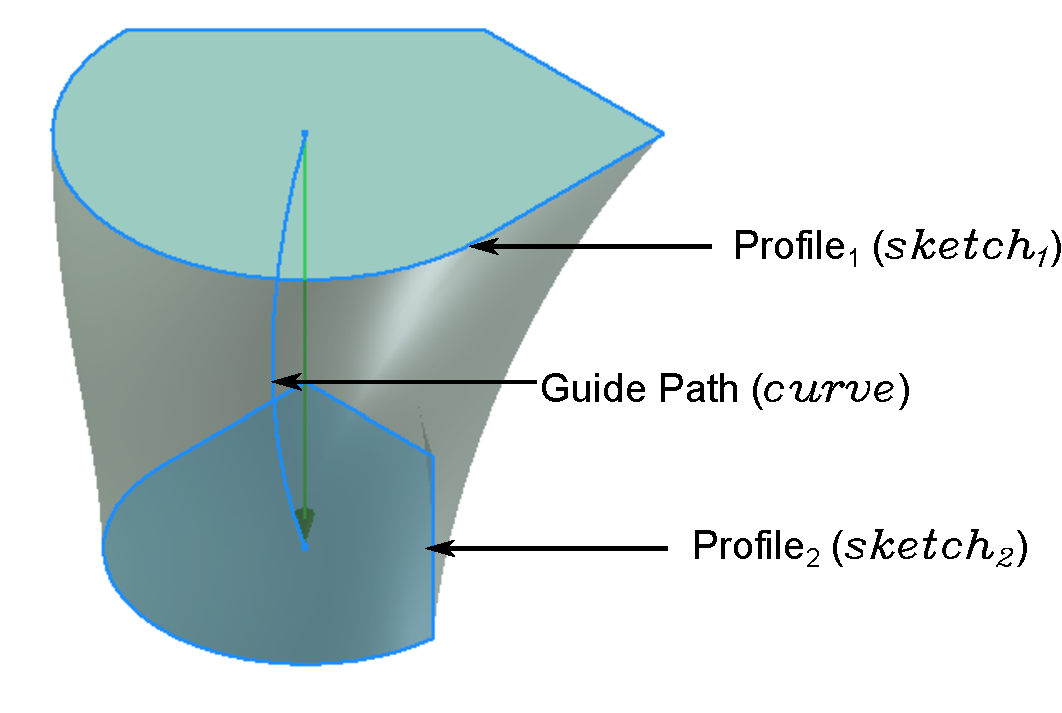
\includegraphics[scale=0.35]{../Common/images//LoftPreview.pdf} 
	%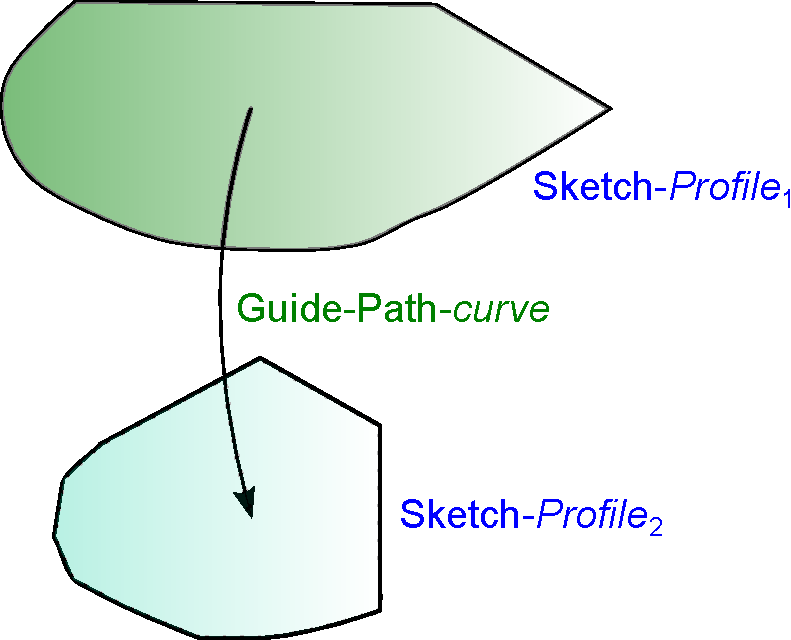
\includegraphics[scale=0.3]{../Common/images//LoftProfilesPath.pdf} \\

%\end{tabular}
\caption{Generic Loft feature}
\label{figure_Loft}
\end{figure}

Represented as:
\loft{}{subtype}{3}{curve, 0 | C_{0,1,2}}{ (sketch )^{<1-n>}}

{\em Continuity} options like $C_0$ for connectedness, $C_1$ for tangency and $C_2$ for curvature continuity can be specified at the ends where body generated by the {\em Loft} joins the existing shape. In case this body is disjoint or is the first one in the scene, no {\em continuity}  is specified. Some form features also specify a {\em draft-angle}  for tapering sides. This can be modeled as {\em Loft} between two {\em profiles}, where the second {\em profile} is offset-ed inside-or-outside. Output of the Loft can either be $solid$ (where capping faces are put to close the shape) or $surface$ (capping faces are not put) and accordingly dimensionality of $2|3$ can be specified.


\begin{figure}[htbp]
	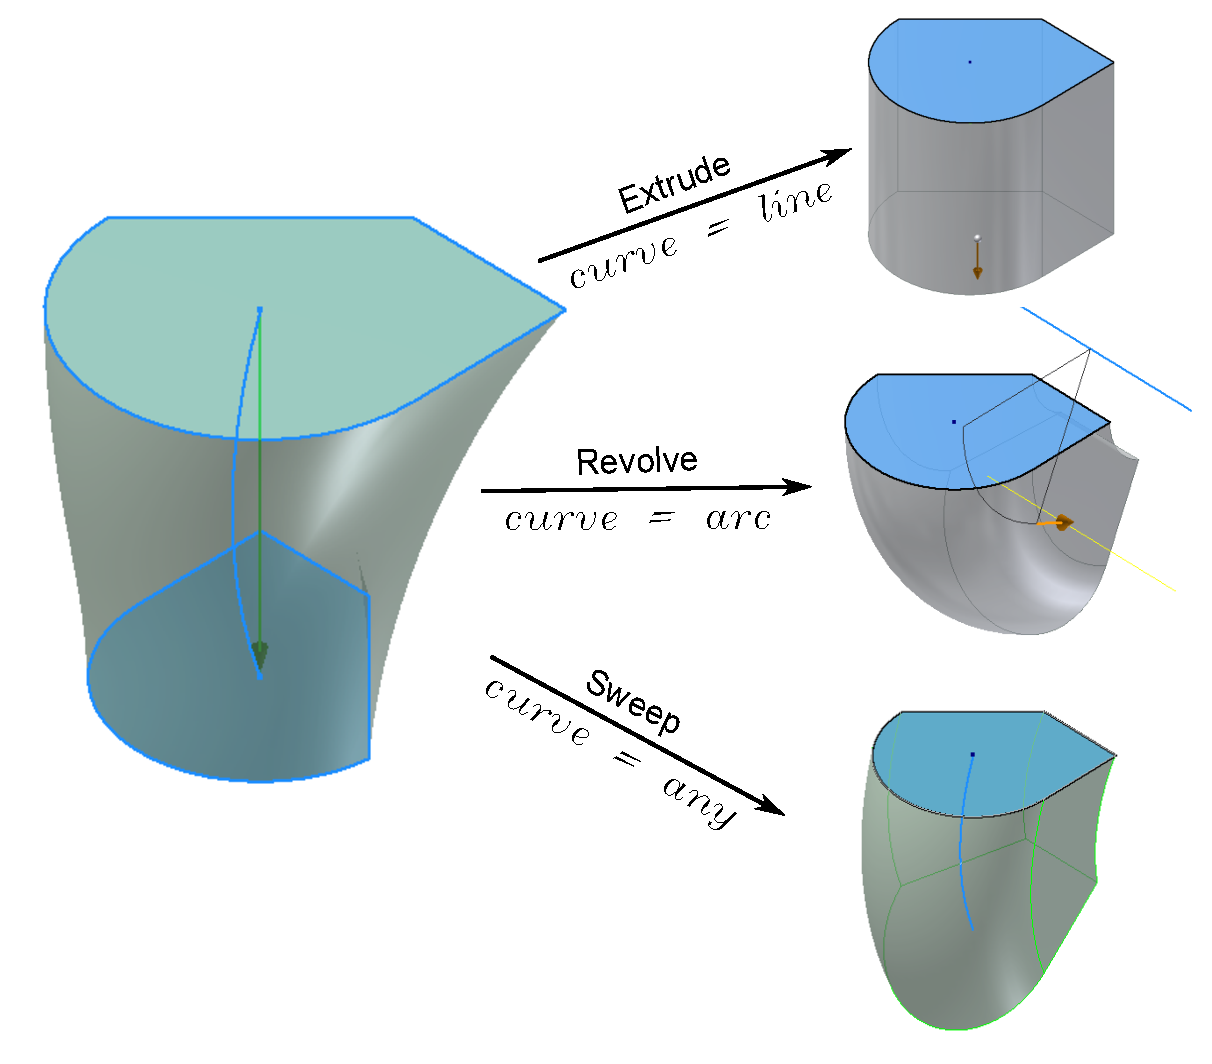
\includegraphics[scale=0.35]{../Common/images//LoftExtrudeRevSwp.pdf} 
\caption{Extrude, Revolve and Sweep in terms of Loft}
\label{figure_extrevswp}
\end{figure}

{\bf Loft} can manifest itself in different forms (Figure \ref{figure_extrevswp}) as elaborated below:
%----------------------------------------------------------------------------------
\begin{itemize}[noitemsep,topsep=2pt,parsep=2pt,partopsep=2pt,label={},leftmargin=*]
\item {\bf Extrude without draft} is denoted by $EnD$ subtype, has single $sketch$, swept along a $line$ and is expressed as	\loft{}{EnD}{3 }{line, 0 | C_0}{ (sketch )^{<1>}}		
\item {\bf Extrude with draft} is denoted by $EwD$ subtype, has two $sketches$ between which loft is made along a $line$ and is expressed as \loft{}{EwD}{3 }{line, 0 | C_0}{ (sketch )^{<1-2>}}	
%\item {\bf Revolve without draft} is denoted by $RnD$ subtype, has single $sketch$, swept along a $arc$ and is expressed as	\loft{}{RnD}{3 }{arc, 0 | C_0}{ (sketch )^{<1>}}		
%\item {\bf Revolve with draft} is denoted by$ RwD$ subtype, has two $sketches$ between which loft is made along a $arc$ and is expressed as\loft{}{RwD}{3 }{arc, 0 | C_0}{ (sketch )^{<1-2>}}	
%\item {\bf Sweep without draft} is denoted by $SnD$ subtype, has single $sketch$, swept along a $curve$ and is expressed as	\loft{}{SnD}{3 }{curve, 0 | C_0}{ (sketch )^{<1>}}		
%\item {\bf Sweep with draft} is denoted by $SwD$ subtype, has two $sketches$ between which loft is made along a $curve$ and is expressed as \loft{}{SwD}{3 }{curve, 0 | C_0}{ (sketch )^{<1-2>}}	
%\item A generic {\bf Loft} is $n$ profiles between which a loft is made along a generic $curve$ and is expressed as \loft{}{L}{3 }{curve, 0 | C_{0,1,2}}{ (sketch )^{<1-n>}} 
\end{itemize}

Similarly {\em Revolve, Sweep, Loft}, with or without draft, can be expressed. {\em Primitive} shapes are further specializations of {\bf $\mathcal{L}$} operators like {\em Extrude} and {\em Revolve}. By changing shape of the {\em profile} and {\em curve} one can get different standard primitives  (Figure \ref{figure_ExtrudeBoxCylCone}) .

\begin{figure}[htbp]
	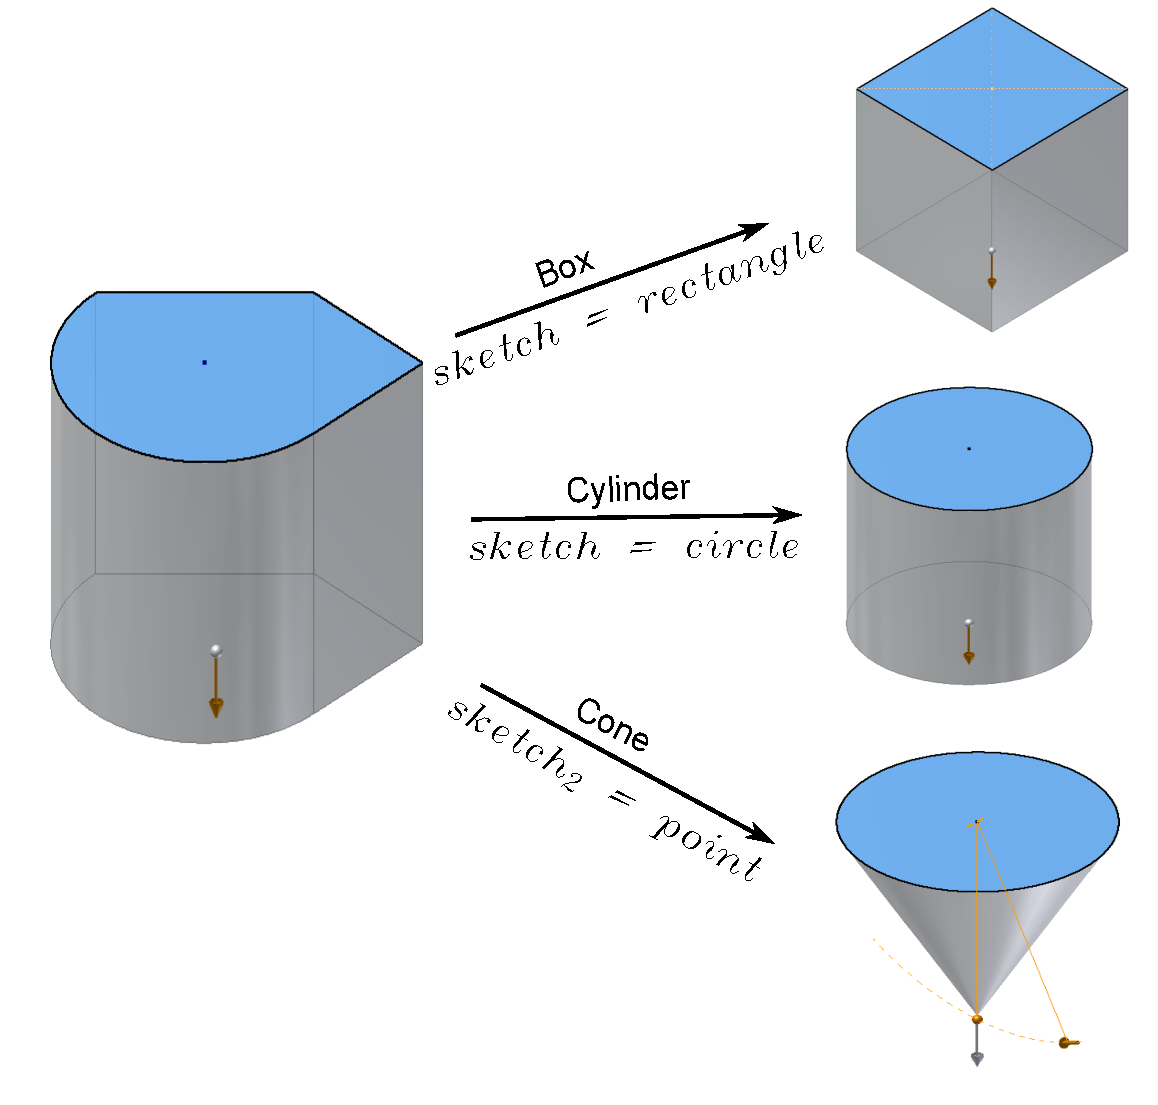
\includegraphics[scale=0.35]{../Common/images//ExtrudeBoxCylCone.pdf} 
\caption{Box, Cylinder, Cone in terms of Extrude-Loft}
\label{figure_ExtrudeBoxCylCone}
\end{figure}
%
%\begin{enumerate}
%\item {\bf Box} : {\em Extrude} with {\em Rectangle} as profile shape and is expressed as \loft{}{EnD}{3 }{line, 0 | C_0}{ (rectangle )}	
%\item {\bf Cylinder} : {\em Extrude} with {\em Circle} as profile shape and is expressed as \loft{}{EnD}{3 }{line, 0 | C_0}{ (circle )}
%\item {\bf Cone}: {\em Extrude with draft} with {\em Circle} as first profile shape, point as second and is expressed as \loft{}{EwD}{3 }{line, 0 | C_0}{ (circle, point)}
%\item {\bf Torus} : {\em Revolve} with {\em Circle} as profile shape, arc as path and is expressed as \loft{}{RnD}{3 }{arc, 0 | C_0}{ (circle)}	
%\item {\bf Sphere} : {\em Revolve} with {\em Circle} as profile shape, point as path and is expressed as \loft{}{RnD}{3 }{point, 0 | C_0}{ (circle)}	
%\end{enumerate}

%---------------------------------------------------------------------------------------------------------------------------------------------------------------------------------
As demonstrated above, most of the form features used in CAD application can be modeled using  three operators, Affine Transformation ($\mathcal{A}$),  Boolean ($\mathcal{B}$) and Loft ($\mathcal{L}$), operating on Entities($\mathcal{E}$). 

This representation is called as {\bf $\mathcal{ABLE}$}.  Other features like {\em Shell, Fillet, Chamfer} can be formulated using {\bf $\mathcal{ABLE}$}. 

%
%\section{Modeling using Point, Transformations, Booleans and Lofts}
%
%With $Point$ as a fundamental entity, other entities and features can be defined using $\mathcal{L}$ (Refer ~\ref{table_ABELTable}).
%\begin{table}[!h]
%\begin{tabular}[h]{@{}p{0.35\linewidth} p{0.18\linewidth} p{0.18\linewidth} p{0.18\linewidth}@{}}
%\toprule
%%\backslashbox[1mm]{sketch}{guide} & {\bf line} & {\bf arc} & {\bf curve}\\
% $sketch\downarrow guide\rightarrow$  & {\bf line} & {\bf arc} & {\bf curve}\\
%\midrule
%point & line & arc & curve \\\midrule
%line & plane surf & cylinder surf & ruled surf\\\midrule
%arc & cylinder surf & torus surf & saddle surf \\\midrule
%open profile & ruled surf & circular surf &  free form surf \\\midrule
%rectangle & box & rect torus & rect sweep \\\midrule
%circle & cylinder (surf/solid) & torus (surf/solid)  & tube (surf/solid) \\\midrule
%closed profile & Extrude  (surf/solid) & Revolve (surf/solid) & Sweep (surf/solid) \\\midrule
%
%%\bottomrule
%\end{tabular}
%\caption{Entities and Features using $\mathcal{L}$}
%\label{table_ABELTable}
%\end{table}
%$\mathcal{L}$oft is more generic case where body is created between more than one sketches along the guide curve. Any arbitrary Free From surface is a network of u-v curves and can be imagined as a $\mathcal{L}$oft of multiple $u$ curves along multiple $v$ curves.
%

\subsubsection{Representing Sheet Metal features using  $\mathcal{ABLE}$}
Sheet Metal parts are modeled, either by using {\em Sketch} based features or by preparing a solid model first and then making it hollow using {\em Shell} operation. The first approach is elaborated below whereas the latter can be treated as subtraction of an offset-ed tool body from the target body. 
%----------------------------------------------------------------------------------
\begin{itemize}[noitemsep,topsep=2pt,parsep=2pt,partopsep=2pt,label={},leftmargin=*]
\item {\bf Face-Wall-Base Flange} can be represented by {\em Extrude} of a given {\em Profile}.
\item {\bf Rib} is a triangular profile extruded.
\item {\bf Hole-Cutout-Slot} is a negative boolean of a tool body which can be represented by  {\em Extrude} of a respective {\em Profile}.
\item {\bf Lance-Louver} is a combination of cut first, then addition of a {\em Sweep} with respective profiles. 
\item {\bf Bend} is a {\em Sweep} of a {\em Rectangular  Profile}	 of edge length. One can add subtype based on the type of relief provided.
\item {\bf Draw-Coin} is a specialized {\em Loft}, with draft, with {\em guide curve} having fillets at the start and end.
\end{itemize}


Following section demonstrates how{\bf $\mathcal{ABLE}$} can be used to express the Midsurface operator.

\subsection{Midsurface using $\mathcal{ABLE}$}

%Most of the Midsurface Extraction algorithms work on geometry of the final shape, which can be in the form of {\em Mesh} or Boundary Representation ({\em Brep}) solid. Midsurfaces generated by these algorithms are still  not well connected and have problems like spurious surfaces, gaps etc. Very few (\cite{Hamdi2005}, \cite{Robinson2006} and \cite{Stolt2005}) have considered leveraging use of feature information in such algorithms, but their usage is limited to very basic form features. Some approaches (\cite{Boussuge2013a}) use decomposition of {\em Brep} solid to create {\em feature tree} like representation so that Midsurface can be worked out on simpler shapes.

In a {\em feature tree}, at each feature level, the operands (especially the {\em tool bodies}) are relatively simpler, thus making Midsurface Extraction more deterministic \cite{YogeshIITM2013}.  Use of Spatial Grammars has made it possible to come up with a terse generic representation (as demonstrated by $\mathcal{ABLE}$) so that algorithms need not have to work on all but just few generic operators. 
%
%As  {\bf $\mathcal{A}$} operators do not change topology and geometry type, Midsurface generated can follow just the same transformation as that of the parent shape. We need to consider only  {\bf $\mathcal{L}$}  and  {\bf $\mathcal{B}$} operators for Midsurface (Figure \ref{figure_Midsurf}) generation. Advantage of the Spatial Grammar defined for Form Features is evident here in the sense one does not need to decide rules for all features but just two - Loft and Boolean, and depending of different specifications they automatically become applicable to rest of the form features.
%
%As for implementation, a {\em feature-based} CAD model is taken as an input. Using direct access or via Application Programming Interface (APIs), {\em feature tree} is queried. A {\em feature tree} is a chronological list of {\em features} stored as part gets built. Each feature is traversed one by one, and wherever applicable, a corresponding Midsurface is extracted. For {\em features} like {\em Extrude} which may have internal-{\em boolean}, two separate {\em features} are modeled, one for {\em tool body} creation by {\em Extrude} and the second one as {\em Boolean}.

For {\em features} based on {\bf $\mathcal{L}$} operator, feature parameters such as {\em sketches-profiles}, {\em curve} etc are extracted first and then, based on the rules specified below, Midsurface is generated.

\begin{itemize}[noitemsep,topsep=2pt,parsep=2pt,partopsep=2pt,label={},leftmargin=*]

\item {\bf Midcurve} is a set of {\em curves} lying midway  of 2D {\em sketch} and is expressed as 	\generic{\Omega}{M}{}{C}{1}{} {sketch} 


\item {\bf Midsurface} rules differ based on the relative sizes of {\em sketch} and {\em curve}.

\begin{itemize}[noitemsep,topsep=2pt,parsep=2pt,partopsep=2pt,label={},leftmargin=*]

\begin{figure}[h]
\centering 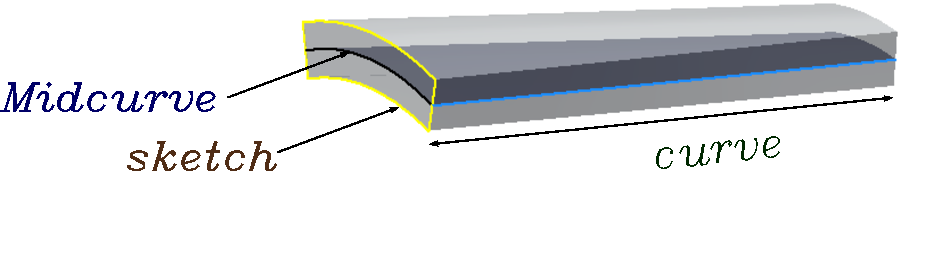
\includegraphics[scale=0.5]{../Common/images//MidsurfSmallProfile.pdf} 
\vspace{-1.5cm}
\caption{sketch is far smaller than curve}
\label{figure_MidsurfSmallProfile}
\end{figure}
\vspace{-0.5cm}

\item {\bf Thin Sketch}: If {\em sketch} is very small compared to {\em curve} ( $sketch_{length} \ll curve_{length}$), then {\em midcurve} is extracted from the {\em sketch} (as mentioned above) and {\em Lofted} with same feature parameters as that of  {\bf $\mathcal{L}$} (Figure \ref{figure_MidsurfSmallProfile}). This rule is expressed as \loft{}{L}{2}{0, curve, 0 | C_{0,1,2}}{midcurve^{1-n}} 

\item {\bf Thin Loft} :  If {\em sketch} is very big compared to {\em curve} ($sketch_{length} \gg curve_{length}$), then {\em midcurve} is not extracted  but the {\em sketch} itself is {\em Lofted} along half of the {\em curve}. This rule is expressed as \loft{}{L}{2}{0, curve/2, 0 | C_{0,1,2}}{sketch}.
%
%\begin{figure}[htbp]
%\centering 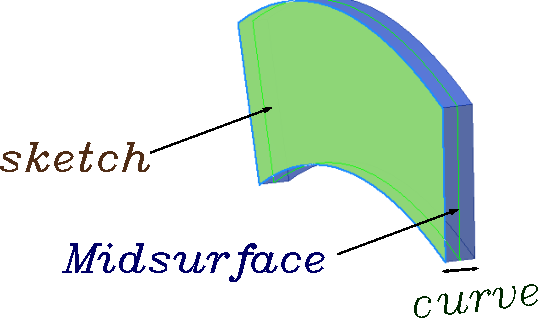
\includegraphics[scale=0.40]{../Common/images//MidsurfSmallCurve.pdf}
%\caption{sketch is far bigger than curve}
%\label{figure_MidsurfSmallCurve}
%\end{figure}

\item {\bf Thick Sketch}:   If {\em sketch} is comparable in size to {\em curve}  ($sketch_{length} \approx curve_{length}$), then it is a thick shape and Midsurface is not generated.
\end{itemize}
\end{itemize}

For {\bf $\mathcal{B}$} operators rules are devised depending on where the target and tools have Midsurface extracted already.
%\vspace{-0.2cm}

\begin{itemize}[noitemsep,topsep=2pt,parsep=2pt,partopsep=2pt,label={},leftmargin=*]

\item {\bf Union} : If the {\em target} and the {\em tool bodies} have Midsurfaces, extend them to join at the common intersections.
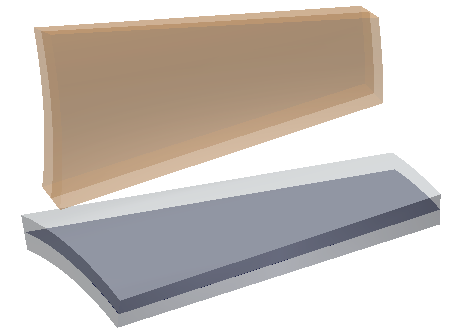
\includegraphics[scale=0.45]{../Common/images//Midsurf_unite.png} 

\item {\bf Difference-Thin} : If the {\em target} has Midsurface then irrespective of {\em tool bodies} being thick or thin, they are subtracted. 
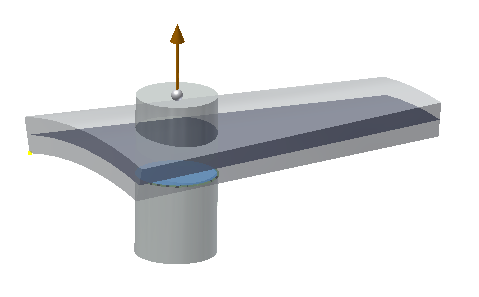
\includegraphics[scale=0.45]{../Common/images//Midsurf_diffthin.png}

\item {\bf Difference-Thick} : If {\em target} and {\em tool bodies} are thick and are in {\em Shell} like situation, {\em midcurves} of combined {\em profiles} are calculated and {\em Lofted}  
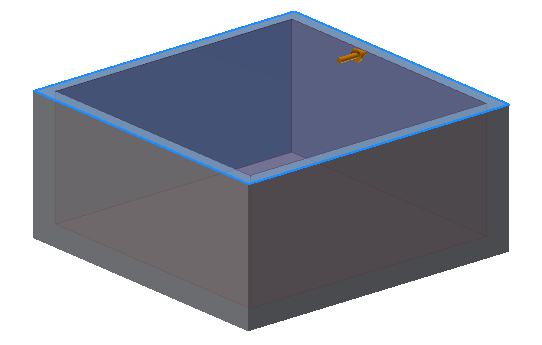
\includegraphics[scale=0.32]{../Common/images//Midsurf_diffthick.png}
\end{itemize}

%\begin{table}[htbp]
%\begin{tabular}{  p{0.3\textwidth} p{0.1\textwidth} }
%
%{\bf Union} : If {\em target} and {\em tool bodies} are thin, extend the Midsurfaces from both and join at common intersection &	
%
%\raisebox{-0.6in}{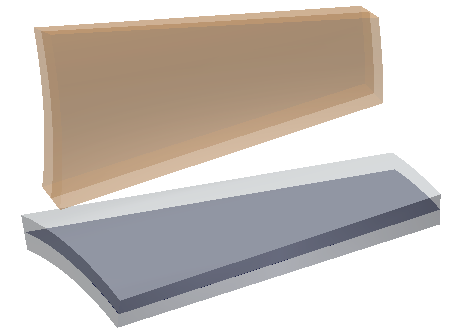
\includegraphics[scale=0.25]{../Common/images//Midsurf_unite.png} } \\
%
%{\bf Difference-Thin} : If {\em target} is thin having Midsurface, then irrespective whether {\em tool bodies} are thick or thin, they cut the Midsurface of {\em target} & 
%
%\raisebox{-0.6in}{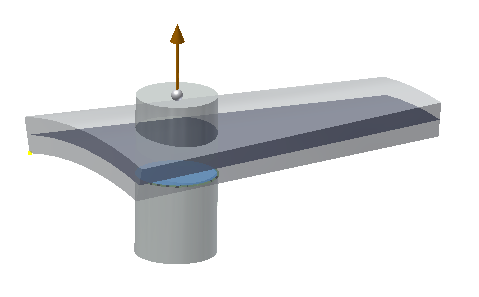
\includegraphics[scale=0.25]{../Common/images//Midsurf_diffthin.png} } \\
%
%{\bf Difference-Thick} : If {\em target} and {\em tool bodies} are thick and are in shell like situation, {\em midcurves} of combined {\em profiles} is calculated and {\em Lofted}  & 
%
%\raisebox{-0.6in}{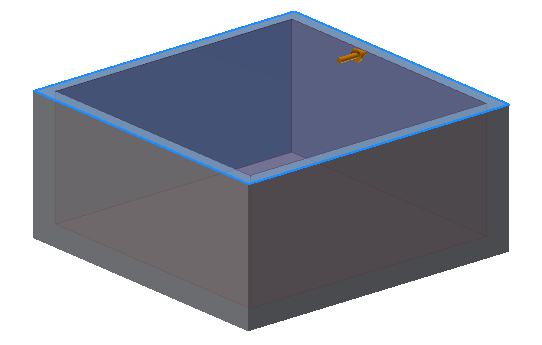
\includegraphics[scale=0.18]{../Common/images//Midsurf_diffthick.png} } \\

%\end{tabular}
%\caption{Midsurface of Boolean Operators}
%\label{table_BoolMidsurf}
%\end{table}



